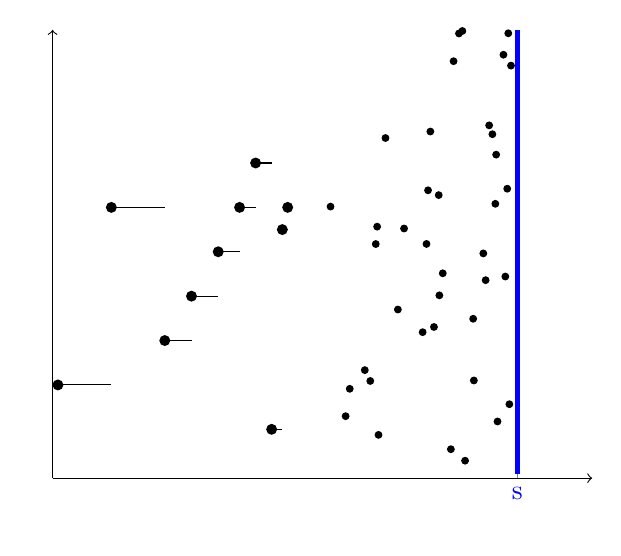
\begin{tikzpicture}[
    declare function={a(\x)=99;},
    declare function={b(\x)=1;}
]%[scale=0.8]
\begin{axis}[
                xlabel=\empty,
                x axis line style={->,opacity=100},
                ylabel=\empty,
                xmin=-1, xmax=100,
                ymin=-1, ymax=100,
                axis y line=left,
                y axis line style={->,opacity=100},
                ytick=\empty,
                xtick={86},
                xticklabel={\textcolor{blue}{s}},
                axis x line*=bottom
                        ]
                        \draw (0,20)--(10,20) node[circle,fill, pos=0,inner sep=1.4pt]{};
                        \draw (10,60)--(20,60) node[circle,fill, pos=0,inner sep=1.4pt]{};
                        \draw (20,30)--(25,30) node[circle,fill, pos=0,inner sep=1.4pt]{};
                        \draw (25,40)--(30,40) node[circle,fill, pos=0,inner sep=1.4pt]{};
                        \draw (30,50)--(34,50) node[circle,fill, pos=0,inner sep=1.4pt]{};
                        \draw (34,60)--(37,60) node[circle,fill, pos=0,inner sep=1.4pt]{};
                        \draw (37,70)--(40,70) node[circle,fill, pos=0,inner sep=1.4pt]{};
                        \draw (40,10)--(42,10) node[circle,fill, pos=0,inner sep=1.4pt]{};
                        \draw (42,55)--(43,55) node[circle,fill, pos=0,inner sep=1.4pt]{};
                        \draw (43,60)--(44,60) node[circle,fill, pos=0,inner sep=1.4pt]{};
                        \addplot [black, domain=50:60, only marks, mark=*, samples=40, mark size=1.2]
    {0.5*(a(x)+b(x)) + 5*rand*(a(x)-b(x))};
                        \addplot [black, domain=60:70, only marks, mark=*, samples=70, mark size=1.2]
    {0.5*(a(x)+b(x)) + 5*rand*(a(x)-b(x))};
                        \addplot [black, domain=70:80, only marks, mark=*, samples=80, mark size=1.2]
    {0.5*(a(x)+b(x)) + 5*rand*(a(x)-b(x))};
    \addplot [black, domain=80:85, only marks, mark=*, samples=100, mark size=1.2]
    {0.5*(a(x)+b(x)) + 5*rand*(a(x)-b(x))};
    \draw[ultra thick,blue](86,0)--(86,100);
\end{axis}
\end{tikzpicture}